\section{Eksperimen}

\subsection{Determinan}
Akan dihitung determinan dari kedua matriks berikut dengan metode matriks kofaktor (MK) dan reduksi baris (RB).

\[ (a) \begin{vmatrix}
1     & 0.5    & 0.333  & 0.25   & 0.2    & 0.166 \\
0.5   & 0.333  & 0.25   & 0.2    & 0.166  & 0.1428 \\
0.333 & 0.25   & 0.2    & 0.166  & 0.1428 & 0.125 \\
0.25  & 0.2    & 0.166  & 0.1428 & 0.125  & 0.111 \\
0.2   & 0.166  & 0.1428 & 0.125  & 0.111  & 0.1 \\
0.166 & 0.1428 & 0.125  & 0.111  & 0.1    & 0.0909 
\end{vmatrix} \qquad (b) 
\begin{vmatrix}
8 & 1 & 3  &2 \\
2 & 9 & -1 & -2 \\
1 & 3 & 2  &-1 \\
1 & 0 & 6  &4 
\end{vmatrix}\]

\begin{lstlisting}[caption = Determinan]
// Masukan
1 0.5 0.333 0.25 0.2 0.166
0.5 0.333 0.25 0.2 0.166 0.1428
0.333 0.25 0.2 0.166 0.1428 0.125
0.25 0.2 0.166 0.1428 0.125 0.111
0.2 0.166 0.1428 0.125 0.111 0.1
0.166 0.1428 0.125 0.111 0.1 0.0909

// Keluaran
Metode Minor Kofaktor:
================== DETERMINAN EKSPANSI KOFAKTOR ==================
Determinan : -9.099246e-13

Metode Reduksi Baris:
================== DETERMINAN METODE REDUKSI BARIS ==================
Determinan : -9.099246e-13
\end{lstlisting}

\begin{lstlisting}[caption = Determinan]
// Masukan
8 1 3 2
2 9 -1 -2
1 3 2 -1
1 0 6 4

// Keluaran
Metode Minor Kofaktor:
================== DETERMINAN EKSPANSI KOFAKTOR ==================
Determinan : 740.000000

Metode Reduksi Baris:
================== DETERMINAN METODE REDUKSI BARIS ==================
Determinan : 740.000000
\end{lstlisting}

\subsection{Invers}

Akan dihitung invers dari kedua matriks berikut dengan metode adjoin maupun metode Gauss-Jordan.

\[(a) \begin{bmatrix}
1     & 0.5    & 0.333  & 0.25   & 0.2    & 0.166 \\
0.5   & 0.333  & 0.25   & 0.2    & 0.166  & 0.1428 \\
0.333 & 0.25   & 0.2    & 0.166  & 0.1428 & 0.125 \\
0.25  & 0.2    & 0.166  & 0.1428 & 0.125  & 0.111 \\
0.2   & 0.166  & 0.1428 & 0.125  & 0.111  & 0.1 \\
0.166 & 0.1428 & 0.125  & 0.111  & 0.1    & 0.0909 
\end{bmatrix} \qquad (b)
\begin{bmatrix}
8  & 1 & 3  & 2 \\
2  & 9 & -1 &  -2 \\
1  & 3 & 2  & -1 \\
1  & 0 & 6  & 4 
\end{bmatrix}
\]

\begin{lstlisting}[caption = Inverse]
// Masukan
1 0.5 0.333 0.25 0.2 0.166
0.5 0.333 0.25 0.2 0.166 0.1428
0.333 0.25 0.2 0.166 0.1428 0.125
0.25 0.2 0.166 0.1428 0.125 0.111
0.2 0.166 0.1428 0.125 0.111 0.1
0.166 0.1428 0.125 0.111 0.1 0.0909

// Keluaran
Metode Gauss Jordan:
================== PENYELESAIAN INVERSE METODE GAUSS JORDAN ==================
[ 6,473229 -20,287200 5,661845 -22,537032 104,428235 -75,098873 ]
[ -20,287200 126,688593 -138,063131 262,713415 -813,216318 601,703831 ]
[ 5,661845 -138,063131 518,917279 -887,920819 962,532452 -481,662764 ]
[ -22,537032 262,713415 -887,920819 698,764686 736,443324 -813,987221 ]
[ 104,428235 -813,216318 962,532452 736,443324 -797,683989 -258,538651 ]
[ -75,098873 601,703831 -481,662764 -813,987221 -258,538651 1143,645743 ]

Metode Adjoin:
================== PENYELESAIAN INVERSE METODE ADJOIN ==================
[ 6,473229 -20,287200 5,661845 -22,537032 104,428235 -75,098873 ]
[ -20,287200 126,688593 -138,063131 262,713415 -813,216318 601,703831 ]
[ 5,661845 -138,063131 518,917279 -887,920819 962,532452 -481,662764 ]
[ -22,537032 262,713415 -887,920819 698,764686 736,443324 -813,987221 ]
[ 104,428235 -813,216318 962,532452 736,443324 -797,683989 -258,538651 ]
[ -75,098873 601,703831 -481,662764 -813,987221 -258,538651 1143,645743 ]
\end{lstlisting}

\begin{lstlisting}[caption = Inverse]
// Masukan
8 1 3 2
2 9 -1 -2
1 3 2 -1
1 0 6 4

// Keluaran
Metode Gauss Jordan:
================== PENYELESAIAN INVERSE METODE GAUSS JORDAN ==================
[ 0,137838 -0,018919 0,010811 -0,075676 ]
[ -0,033784 0,141892 -0,081081 0,067568 ]
[ -0,020270 -0,114865 0,351351 0,040541 ]
[ -0,004054 0,177027 -0,529730 0,208108 ]

Metode Adjoin:
================== PENYELESAIAN INVERSE METODE ADJOIN ==================
[ 0,137838 -0,018919 0,010811 -0,075676 ]
[ -0,033784 0,141892 -0,081081 0,067568 ]
[ -0,020270 -0,114865 0,351351 0,040541 ]
[ -0,004054 0,177027 -0,529730 0,208108 ]
\end{lstlisting}
\pagebreak

\subsection{SPL-1}
Tentukan solusi dari SPL $A\textbf{x} = \textbf{b}$ berikut.

\begin{enumerate}[label=(\alph*)]
    \item
    \[A = \begin{bmatrix}
    1 & 1 & -1 & -1 \\
    2 & 5 & -7 & -5 \\
    2 & -1 & 1 & 3 \\
    5 & 2 & -4 & 2
\end{bmatrix}, \quad b = 
\begin{bmatrix}
    1 \\ -2 \\ 4 \\ 6
\end{bmatrix}\]

    \begin{lstlisting}[caption = spl-1a.txt]
// Masukan
1 1 -1 -1 1
2 5 -7 -5 -2
2 -1 1 3 4
5 2 -4 2 6

// Keluaran
Metode Reduksi Gauss:
================== PENYELESAIAN SPL METODE GAUSS ==================
Solusi tidak dapat ditentukan

Metode Reduksi Gauss-Jordan:
================== PENYELESAIAN SPL METODE GAUSS JORDAN ==================
Solusi tidak dapat ditentukan

Metode Cramer:
================== PENYELESAIAN SPL METODE CRAMER ==================
Solusi tidak dapat ditentukan

Metode Matriks Balikan:
================== PENYELESAIAN SPL METODE BALIKAN ==================
Solusi tidak dapat ditentukan\end{lstlisting}

Keluaran yang diperoleh menunjukkan bahwa solusi tidak dapat ditentukan oleh keempat metode penyelesaian SPL (Metode Reduksi Gauss, Reduksi Gauss-Jordan, Cramer, dan Matriks Balikan). Hal ini disebabkan oleh determinan dari matriks koefisien yang bernilai nol. Ketika determinan dari matriks koefisien sama dengan nol, ini berarti matriks tersebut tidak dapat di-invers, yang menyebabkan sistem persamaan tidak memiliki solusi tunggal atau konsisten. Dalam kasus ini, sistem tidak memiliki solusi tak hingga (parametrik) sehingga tidak memiliki solusi sama sekali (inkonsisten). Oleh karena itu, keluaran program yang menyatakan bahwa solusi tidak dapat ditentukan adalah benar dan sesuai dengan sifat matematis dari SPL tersebut.

\pagebreak
    \item
    \[ A = \begin{bmatrix}
    1 & -1 & 0 & 0 & 1 \\
    1 & 1 & 0 & -3 & 0 \\
    2 & -1 & 0 & 1 & -1 \\
    -1 & 2 & 0 & -2 & -1
\end{bmatrix}, \quad b =
\begin{bmatrix}
    3 \\ 6 \\ 5 \\ -1
\end{bmatrix}\]

\begin{lstlisting}[caption = spl-1b.txt]
// Masukan
1 -1 0 0 1 3
1 1 0 -3 0 6
2 -1 0 1 -1 5
-1 2 0 -2 -1 -1

// Keluaran
Metode Reduksi Gauss:
================== PENYELESAIAN SPL METODE GAUSS ==================
X1 = 3,000000 + 1,000000a2 + -1,000000a5
X2 = 1,500000 + 1,500000a4 + 0,500000a5
X3 = a3
X4 = -1,000000 + 1,000000a5
X5 = a5

Metode Reduksi Gauss-Jordan:
================= PENYELESAIAN SPL METODE GAUSS JORDAN ==================
X1 = 3,000000 + 1,000000a5
X2 = 0,000000 + 2,000000a5
X3 = a3
X4 = -1,000000 + 1,000000a5
X5 = a5

Metode Cramer:
================== PENYELESAIAN SPL METODE CRAMER ==================
SPL tidak dapat dikerjakan dengan metode ini.

Metode Matriks Balikan:
================== PENYELESAIAN SPL METODE BALIKAN ==================
SPL tidak dapat dikerjakan dengan metode ini.\end{lstlisting}

Keluaran dari program menunjukkan bahwa solusi dari sistem persamaan linear ini bervariasi bergantung pada metode yang digunakan. Berikut adalah penjelasan mengenai masing-masing metode:

\textbf{Metode Reduksi Gauss}: Hasil keluaran menunjukkan bahwa sistem memiliki solusi parametrik, di mana variabel \( X_1 \), \( X_2 \), \( X_3 \), \( X_4 \), dan \( X_5 \) dinyatakan dalam bentuk parameter bebas (\( a_2 \), \( a_3 \), \( a_4 \), dan \( a_5 \)). Ini menunjukkan bahwa sistem memiliki banyak solusi, karena beberapa variabel bergantung pada nilai parameter bebas. Artinya, ada kebebasan dalam menentukan nilai beberapa variabel, sehingga menghasilkan solusi parametrik.

\textbf{Metode Reduksi Gauss-Jordan}: Hasil dari metode ini juga menghasilkan solusi parametrik, namun dalam bentuk yang lebih sederhana. Variabel \( X_1 \), \( X_2 \), \( X_3 \), \( X_4 \), dan \( X_5 \) juga dinyatakan dalam bentuk parameter bebas (\( a_3 \) dan \( a_5 \)), tetapi dengan lebih sedikit ketergantungan pada parameter. Solusi ini menunjukkan bahwa sistem masih memiliki banyak solusi, tetapi lebih sederhana dibandingkan hasil dari metode Gauss.

\textbf{Metode Cramer}: Solusi tidak dapat ditentukan menggunakan metode Cramer karena dimensi dari matriks bukan \(n \times (n+1)\). Dalam metode Cramer, kita memerlukan determinan dari matriks koefisien yang berbentuk \(n \times n\).

\textbf{Metode Matriks Balikan}: Solusi juga tidak dapat ditentukan menggunakan metode ini karena dimensi dari matriks bukan \(n \times (n+1)\). Dalam metode Matriks Balikan, kita memerlukan determinan dari matriks koefisien yang bisa di-invers, yang juga mengharuskan matriks berbentuk \(n \times n\).

\pagebreak
    \item 
    \[ A = \begin{bmatrix}
    0 & 1 & 0 & 0 & 1 & 0 \\
    0 & 0 & 0 & 1 & 1 & 0 \\
    0 & 1 & 0 & 0 & 0 & 1 \\
\end{bmatrix}, \quad b =
\begin{bmatrix}
    2 \\ -1 \\ 1
\end{bmatrix}\]

\begin{lstlisting}[caption = spl-1c.txt]
// Masukan
0 1 0 0 1 0 2
0 0 0 1 1 0 -1
0 1 0 0 0 1 1

// Keluaran
Metode Reduksi Gauss:
================== PENYELESAIAN SPL METODE GAUSS ==================
X1 = a1
X2 = 2,000000 + -1,000000a5
X3 = a3
X4 = -1,000000 + -1,000000a5
X5 = 1,000000 + 1,000000a6
X6 = a6

Metode Reduksi Gauss-Jordan:
================= PENYELESAIAN SPL METODE GAUSS JORDAN ==================
X1 = a1
X2 = 1,000000 + -1,000000a6
X3 = a3
X4 = -2,000000 + -1,000000a6
X5 = 1,000000 + 1,000000a6
X6 = a6

Metode Cramer:
================== PENYELESAIAN SPL METODE CRAMER ==================
SPL tidak dapat dikerjakan dengan metode ini.

Metode Matriks Balikan:
================== PENYELESAIAN SPL METODE BALIKAN ==================
SSPL tidak dapat dikerjakan dengan metode ini.\end{lstlisting}

Keluaran dari program menunjukkan hasil sebagai berikut:

\textbf{Metode Reduksi Gauss}: Sistem menghasilkan solusi parametrik. Variabel \( X_1 \), \( X_2 \), \( X_3 \), \( X_4 \), \( X_5 \), dan \( X_6 \) dinyatakan dalam bentuk parameter bebas (\( a_1 \), \( a_3 \), \( a_5 \), dan \( a_6 \)), yang berarti terdapat banyak solusi karena beberapa variabel bergantung pada nilai parameter bebas.

\textbf{Metode Reduksi Gauss-Jordan}: Solusi parametrik yang lebih sederhana dibandingkan metode Gauss, tetapi masih bergantung pada parameter bebas \( a_1 \), \( a_3 \), dan \( a_6 \). Sistem masih memiliki banyak solusi yang tergantung pada nilai parameter tersebut.

\textbf{Metode Cramer}: Solusi tidak dapat ditentukan menggunakan metode Cramer karena dimensi dari matriks bukan \(n \times (n+1)\). 

\textbf{Metode Matriks Balikan}: Solusi juga tidak dapat ditentukan menggunakan metode ini karena dimensi dari matriks bukan \(n \times (n+1)\).

\pagebreak
\item Uji untuk $n = 6$ dan $n = 11$.
\[ A = H = \begin{bmatrix}
    1               & \dfrac{1}{2}   & \dfrac{1}{3}   & \ldots & \dfrac{1}{n}     \\[1em]
    \dfrac{1}{2}    & \dfrac{1}{3}   & \dfrac{1}{4}   & \ldots & \dfrac{1}{n+1}   \\[1em]
    \dfrac{1}{3}    & \dfrac{1}{4}   & \dfrac{1}{5}   & \ldots & \dfrac{1}{n+2}   \\[1em]
    \vdots          & \vdots         & \vdots         & \ddots & \vdots           \\[1em]
    \dfrac{1}{n}    & \dfrac{1}{n+1} & \dfrac{1}{n+2} & \ldots & \dfrac{1}{2n-1}\\
\end{bmatrix}, \quad b =
\begin{bmatrix}
    1 \\ 0 \\ 0 \\ \ldots \\ 0
\end{bmatrix}\]

\begin{lstlisting}[caption = spl-1d1.txt]
// Masukan
1.000000 0.500000 0.333333 0.250000 0.200000 0.166667 1
0.500000 0.333333 0.250000 0.200000 0.166667 0.142857 0
0.333333 0.250000 0.200000 0.166667 0.142857 0.125000 0
0.250000 0.200000 0.166667 0.142857 0.125000 0.111111 0
0.200000 0.166667 0.142857 0.125000 0.111111 0.100000 0
0.166667 0.142857 0.125000 0.111111 0.100000 0.090909 0

// Keluaran
Metode Reduksi Gauss:
================== PENYELESAIAN SPL METODE GAUSS ==================
X1 = 11,540412
X2 = 46,616694
X3 = -1130,944969
X4 = 3969,618023
X5 = -5045,250153
X6 = 2158,663954

Metode Reduksi Gauss-Jordan:
================= PENYELESAIAN SPL METODE GAUSS JORDAN ==================
X1 = 11,540412
X2 = 46,616694
X3 = -1130,944969
X4 = 3969,618023
X5 = -5045,250153
X6 = 2158,663954

Metode Cramer:
================== PENYELESAIAN SPL METODE CRAMER ==================
X1 = 11,540412
X2 = 46,616694
X3 = -1130,944969
X4 = 3969,618023
X5 = -5045,250153
X6 = 2158,663954

Metode Matriks Balikan:
================== PENYELESAIAN SPL METODE BALIKAN ==================
X1: 11,540412
X2: 46,616694
X3: -1130,944969
X4: 3969,618023
X5: -5045,250153
X6: 2158,663954\end{lstlisting}

\begin{lstlisting}[caption = spl-1d2.txt]
// Masukan
1.000000 0.500000 0.333333 0.250000 0.200000 0.166667 0.142857 0.125000 0.111111 0.100000 1
0.500000 0.333333 0.250000 0.200000 0.166667 0.142857 0.125000 0.111111 0.100000 0.090909 0
0.333333 0.250000 0.200000 0.166667 0.142857 0.125000 0.111111 0.100000 0.090909 0.083333 0
0.250000 0.200000 0.166667 0.142857 0.125000 0.111111 0.100000 0.090909 0.083333 0.076923 0
0.200000 0.166667 0.142857 0.125000 0.111111 0.100000 0.090909 0.083333 0.076923 0.071429 0
0.166667 0.142857 0.125000 0.111111 0.100000 0.090909 0.083333 0.076923 0.071429 0.066667 0
0.142857 0.125000 0.111111 0.100000 0.090909 0.083333 0.076923 0.071429 0.066667 0.062500 0
0.125000 0.111111 0.100000 0.090909 0.083333 0.076923 0.071429 0.066667 0.062500 0.058824 0
0.111111 0.100000 0.090909 0.083333 0.076923 0.071429 0.066667 0.062500 0.058824 0.055556 0
0.100000 0.090909 0.083333 0.076923 0.071429 0.066667 0.062500 0.058824 0.055556 0.052632 0

// Keluaran
Metode Reduksi Gauss:
================== PENYELESAIAN SPL METODE GAUSS ==================
X1 = 19,525627
X2 = -159,545670
X3 = 20,759112
X4 = 1983,940776
X5 = -5084,976735
X6 = 5660,147295
X7 = -4622,220507
X8 = 3257,960172
X9 = -623,836012
X10 = -456,355282

Metode Reduksi Gauss-Jordan:
================= PENYELESAIAN SPL METODE GAUSS JORDAN ==================
X1 = 19,525627
X2 = -159,545670
X3 = 20,759112
X4 = 1983,940776
X5 = -5084,976735
X6 = 5660,147295
X7 = -4622,220507
X8 = 3257,960172
X9 = -623,836012
X10 = -456,355282

Metode Cramer:
================== PENYELESAIAN SPL METODE CRAMER ==================
X1 = 19,525627
X2 = -159,545670
X3 = 20,759112
X4 = 1983,940776
X5 = -5084,976735
X6 = 5660,147295
X7 = -4622,220507
X8 = 3257,960172
X9 = -623,836012
X10 = -456,355282

Metode Matriks Balikan:
================== PENYELESAIAN SPL METODE BALIKAN ==================
X1: 19,525627
X2: -159,545670
X3: 20,759112
X4: 1983,940776
X5: -5084,976735
X6: 5660,147295
X7: -4622,220507
X8: 3257,960172
X9: -623,836012
X10: -456,355282\end{lstlisting}

\end{enumerate}

Keluaran program menunjukkan bahwa sistem persamaan linear yang diberikan memiliki solusi unik, dan keempat metode yang digunakan (Metode Reduksi Gauss, Reduksi Gauss-Jordan, Metode Cramer, dan Matriks Balikan) menghasilkan solusi yang sama. Dapat disimpulkan bahwa sistem ini memiliki determinan matriks koefisien tidak nol, memungkinkan metode eliminasi, Cramer, dan matriks balikan untuk memberikan solusi yang sama.

\pagebreak
\subsection{SPL-2}
Selesaikan SPL berbentuk matriks \textit{augmented} berikut.

\[(a) \begin{bmatrix}
1 & -1 & 2 & -1 & -1\\
2 & 1 & -2 & -2 & -2\\
-1 & 2 & -4 & 1 & 1 \\
3 & 0 & 0 & -3 & -3 
\end{bmatrix} \qquad (b)
\begin{bmatrix}
2   & 0  & 8  & 0  & 8  \\
0   & 1  & 0  & 4  & 6  \\
-4  & 0  & 6  & 0  & 6  \\
0   & -2 & 0  & 3  & -1 \\
2   & 0  & -4 & 0  & -4 \\
0   & 1  & 0  & -2 & 0
\end{bmatrix}\]

\begin{lstlisting}[caption = spl-2a.txt]
// Masukan
1 -1 2 -1 -1
2 1 -2 -2 -2
-1 2 -4 1 1
3 0 0 -3 -3

// Keluaran
Metode Reduksi Gauss:
================== PENYELESAIAN SPL METODE GAUSS ==================
X1 = -1,000000 + 1,000000a2 + -2,000000a3 + 1,000000a4
X2 = 0,000000 + 2,000000a3
X3 = a3
X4 = a4

Metode Reduksi Gauss-Jordan:
================= PENYELESAIAN SPL METODE GAUSS JORDAN ==================
X1 = -1,000000 + 1,000000a4
X2 = 0,000000 + 2,000000a3
X3 = a3
X4 = a4

Metode Cramer:
================== PENYELESAIAN SPL METODE CRAMER ==================
Solusi tidak dapat ditentukan

Metode Matriks Balikan:
================== PENYELESAIAN SPL METODE BALIKAN ==================
Solusi tidak dapat ditentukan\end{lstlisting}

Di sini kaidah Cramer dan metode Matriks Balikan tidak dapat memberikan solusi akibat determinan dari matriks adalah 0

\begin{lstlisting}[caption = spl-2b.txt]
// Masukan
2 0 8 0 8
0 1 0 4 6
-4 0 6 0 6
0 -2 0 3 -1
2 0 -4 0 -4
0 1 0 -2 0

// Keluaran
Metode Reduksi Gauss:
================== PENYELESAIAN SPL METODE GAUSS ==================
X1 = 0,000000
X2 = 2,000000
X3 = 1,000000
X4 = 1,000000

Metode Reduksi Gauss-Jordan:
================= PENYELESAIAN SPL METODE GAUSS JORDAN ==================
X1 = 0,000000
X2 = 2,000000
X3 = 1,000000
X4 = 1,000000

Metode Cramer:
================== PENYELESAIAN SPL METODE CRAMER ==================
SPL tidak dapat dikerjakan dengan metode ini.

Metode Matriks Balikan:
================== PENYELESAIAN SPL METODE BALIKAN ==================
SPL tidak dapat dikerjakan dengan metode ini.\end{lstlisting}

Di sini kaidah Cramer dan metode Matriks Balikan tidak dapat digunakan karena banyaknya persamaan tidak sama dengan banyaknya peubah, atau dengan kata lain matriks koefisien bukan matriks persegi sehingga tidak memiliki determinan.

\pagebreak
\subsection{SPL-3}
\begin{enumerate}[label=(\alph*)]
    \item 
\begin{align*}
    8x_1 + x_2 + 3x_3 + 2x_4 &= 0 \\
    2x_1 + 9x_2 - x_3 - 2x_4 &= 1 \\
    x_1 + 3x_2 + 2x_3 - x_4 &= 2 \\
    x_1 + 6x_3 + 4x_4 &= 3
\end{align*}

\begin{lstlisting}[caption = spl-3a.txt]
// Masukan
8 1 3 2 0
2 9 -1 -2 1
1 3 2 -1 2
1 0 6 4 3

// Keluaran
Metode Reduksi Gauss:
================== PENYELESAIAN SPL METODE GAUSS ==================
X1 = -0,224324
X2 = 0,182432
X3 = 0,709459
X4 = -0,258108

Metode Reduksi Gauss-Jordan:
================= PENYELESAIAN SPL METODE GAUSS JORDAN ==================
X1 = -0,224324
X2 = 0,182432
X3 = 0,709459
X4 = -0,258108

Metode Cramer:
================== PENYELESAIAN SPL METODE CRAMER ==================
X1 = -0,224324
X2 = 0,182432
X3 = 0,709459
X4 = -0,258108

Metode Matriks Balikan:
================== PENYELESAIAN SPL METODE BALIKAN ==================
X1: -0,224324
X2: 0,182432
X3: 0,709459
X4: -0,258108\end{lstlisting}

Keluaran program menunjukkan bahwa sistem persamaan linear yang diberikan memiliki solusi unik, dan keempat metode yang digunakan (Metode Reduksi Gauss, Reduksi Gauss-Jordan, Metode Cramer, dan Matriks Balikan) menghasilkan solusi yang sama. Dapat disimpulkan bahwa sistem ini memiliki determinan matriks koefisien tidak nol, memungkinkan metode eliminasi, Cramer, dan matriks balikan untuk memberikan solusi yang sama.

\pagebreak
    \item
\begin{align*}
    x_7 + x_8 + x_9 &= 13.00 \\
    x_4 + x_5 + x_6 &= 15.00 \\
    x_1 + x_2 + x_3 &= 8.00 \\
    0.04289(x_3 + x_5 + x_7) + 0.75(x_6 + x_8) + 0.61396x_9 &= 14.79 \\
    0.91421(x_3 + x_5 + x_7) + 0.25(x_2 + x_4 + x_6 + x_8) &= 14.31 \\
    0.04289(x_3 + x_5 + x_7) + 0.75(x_2 + x_4) + 0.61396x_1 &= 3.81 \\
    x_3 + x_6 + x_9 &= 18.00 \\
    x_2 + x_5 + x_8 &= 12.00 \\
    x_1 + x_4 + x_7 &= 6.00 \\
    0.04289(x_1 + x_5 + x_9) + 0.75(x_2 + x_6) + 0.61396x_3 &= 10.51\\
    0.91421(x_1 + x_5 + x_9) + 0.25(x_2 + x_4 + x_6 + x_8) &= 16.13 \\
    0.04289(x_1 + x_5 + x_9) + 0.75(x_4 + x_8) + 0.61396x_7 &= 7.04
\end{align*}

\begin{lstlisting}[caption = spl-3b.txt]
// Masukan
0 0 0 0 0 0 1 1 1 13.00
0 0 0 1 1 1 0 0 0 15.00
1 1 1 0 0 0 0 0 0 8.00
0 0 0.04289 0 0.04289 0.75 0.04289 0.75 0.61396 14.79
0 0.25 0.91421 0.25 0.91421 0.25 0.91421 0.25 0 14.31
0.61396 0.75 0.04289 0.75 0.04289 0 0.04289 0 0 3.81
0 0 1 0 0 1 0 0 1 18.00
0 1 0 0 1 0 0 1 0 12.00
1 0 0 1 0 0 1 0 0 6.00
0.04289 0.75 0.61396 0 0.04289 0.75 0 0 0.04289 10.51
0.91421 0.25 0 0.25 0.91421 0.25 0 0.25 0.91421 16.13
0.04289 0 0 0.75 0.04289 0 0.61396 0.75 0.04289 7.04

// Keluaran
Metode Reduksi Gauss:
================== PENYELESAIAN SPL METODE GAUSS ==================
Solusi tidak dapat ditentukan

Metode Reduksi Gauss-Jordan:
================= PENYELESAIAN SPL METODE GAUSS JORDAN ==================
Solusi tidak dapat ditentukan

Metode Cramer:
================== PENYELESAIAN SPL METODE CRAMER ==================
SPL tidak dapat dikerjakan dengan metode ini.

Metode Matriks Balikan:
================== PENYELESAIAN SPL METODE BALIKAN ==================
SPL tidak dapat dikerjakan dengan metode ini.\end{lstlisting}

Untuk metode Gauss dan Gauss-Jordan, tidak ada solusi karena setelah reduksi, terdapat baris di mana kolom paling akhir memiliki nilai, sedangkan kolom-kolom lainnya pada baris yang sama bernilai 0 semua. Ini menunjukkan adanya ketidakkonsistenan, di mana persamaan tersebut tidak mungkin dipenuhi, sehingga sistem persamaan tidak memiliki solusi. Metode Cramer dan Matriks Balikan tidak dapat ditentukan karena banyaknya persamaan tidak sama dengan banyaknya peubah, atau dengan kata lain matriks koefisien bukan matriks persegi sehingga tidak memiliki determinan.

\end{enumerate}
\pagebreak
\subsection{SPL-4}
Lihatlah sistem reaktor pada gambar berikut.

{\centering

\begin{figure}
    \centering
\tikzset{every picture/.style={line width=0.75pt}} %set default line width to 0.75pt        
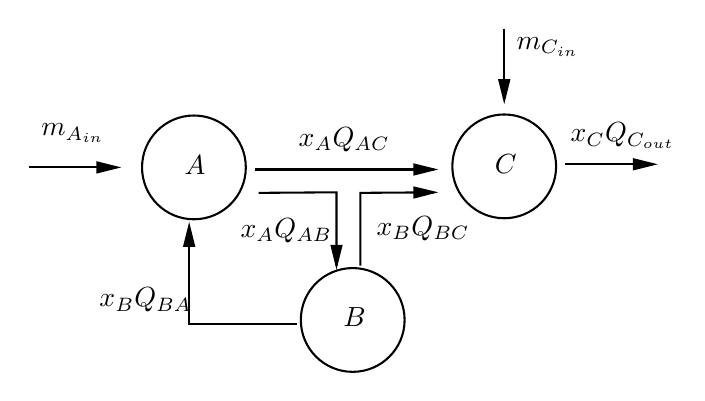
\begin{tikzpicture}[x=0.75pt,y=0.75pt,yscale=-1,xscale=1]
%uncomment if require: \path (0,300); %set diagram left start at 0, and has height of 300

%Shape: Circle [id:dp6473343373803122] 
\draw   (136,74.5) .. controls (136,60.69) and (147.19,49.5) .. (161,49.5) .. controls (174.81,49.5) and (186,60.69) .. (186,74.5) .. controls (186,88.31) and (174.81,99.5) .. (161,99.5) .. controls (147.19,99.5) and (136,88.31) .. (136,74.5) -- cycle ;

%Straight Lines [id:da45667048163316837] 
\draw    (81.4,74.5) -- (124,74.5) ;
\draw [shift={(126,74.5)}, rotate = 180] [fill={rgb, 255:red, 0; green, 0; blue, 0 }  ][line width=0.08]  [draw opacity=0] (12,-3) -- (0,0) -- (12,3) -- cycle    ;
%Shape: Circle [id:dp10276116991385953] 
\draw   (285.5,74) .. controls (285.5,60.19) and (296.69,49) .. (310.5,49) .. controls (324.31,49) and (335.5,60.19) .. (335.5,74) .. controls (335.5,87.81) and (324.31,99) .. (310.5,99) .. controls (296.69,99) and (285.5,87.81) .. (285.5,74) -- cycle ;

%Shape: Circle [id:dp5407854717024974] 
\draw   (212.5,148) .. controls (212.5,134.19) and (223.69,123) .. (237.5,123) .. controls (251.31,123) and (262.5,134.19) .. (262.5,148) .. controls (262.5,161.81) and (251.31,173) .. (237.5,173) .. controls (223.69,173) and (212.5,161.81) .. (212.5,148) -- cycle ;

%Straight Lines [id:da8849136386389991] 
\draw    (339.9,73) -- (382.5,73) ;
\draw [shift={(384.5,73)}, rotate = 180] [fill={rgb, 255:red, 0; green, 0; blue, 0 }  ][line width=0.08]  [draw opacity=0] (12,-3) -- (0,0) -- (12,3) -- cycle    ;
%Straight Lines [id:da8406763034964528] 
\draw    (310.5,7.68) -- (310.5,42) ;
\draw [shift={(310.5,44)}, rotate = 270] [fill={rgb, 255:red, 0; green, 0; blue, 0 }  ][line width=0.08]  [draw opacity=0] (12,-3) -- (0,0) -- (12,3) -- cycle    ;
%Straight Lines [id:da28568694217154267] 
\draw    (190.4,75.5) -- (276.7,75.5) ;
\draw [shift={(278.7,75.5)}, rotate = 180] [fill={rgb, 255:red, 0; green, 0; blue, 0 }  ][line width=0.08]  [draw opacity=0] (12,-3) -- (0,0) -- (12,3) -- cycle    ;
%Straight Lines [id:da9310039435647144] 
\draw    (241.2,121.77) -- (241.2,86.77) -- (276.7,86.51) ;
\draw [shift={(278.7,86.5)}, rotate = 179.58] [fill={rgb, 255:red, 0; green, 0; blue, 0 }  ][line width=0.08]  [draw opacity=0] (12,-3) -- (0,0) -- (12,3) -- cycle    ;
%Straight Lines [id:da924484609130307] 
\draw    (192.2,86.77) -- (229.7,86.5) -- (229.7,121.77) ;
\draw [shift={(229.7,123.77)}, rotate = 270] [fill={rgb, 255:red, 0; green, 0; blue, 0 }  ][line width=0.08]  [draw opacity=0] (12,-3) -- (0,0) -- (12,3) -- cycle    ;
%Straight Lines [id:da12490409145537429] 
\draw    (210.5,150) -- (158.7,150) -- (158.7,102.77) ;
\draw [shift={(158.7,100.77)}, rotate = 90] [fill={rgb, 255:red, 0; green, 0; blue, 0 }  ][line width=0.08]  [draw opacity=0] (12,-3) -- (0,0) -- (12,3) -- cycle    ;

% Text Node
\draw (86,52.1) node [anchor=north west][inner sep=0.75pt]    {$m_{A_{in}}$};
% Text Node
\draw (155,67.1) node [anchor=north west][inner sep=0.75pt]    {$A$};
% Text Node
\draw (304.5,66.6) node [anchor=north west][inner sep=0.75pt]    {$C$};
% Text Node
\draw (231.5,140.6) node [anchor=north west][inner sep=0.75pt]    {$B$};
% Text Node
\draw (341,51.6) node [anchor=north west][inner sep=0.75pt]    {$x_{C} Q_{C_{out}}$};
% Text Node
\draw (315,10.6) node [anchor=north west][inner sep=0.75pt]    {$m_{C_{in}}$};
% Text Node
\draw (210,53.6) node [anchor=north west][inner sep=0.75pt]    {$x_{A} Q_{AC}$};
% Text Node
\draw (247.5,96.6) node [anchor=north west][inner sep=0.75pt]    {$x_{B} Q_{BC}$};
% Text Node
\draw (182,97.6) node [anchor=north west][inner sep=0.75pt]    {$x_{A} Q_{AB}$};
% Text Node
\draw (114,131.1) node [anchor=north west][inner sep=0.75pt]    {$x_{B} Q_{BA}$};


\end{tikzpicture}
    \caption{Model rangkaian reaktor}
\end{figure}
\par}

Dengan laju volume $Q$ dalam m$^3$/s dan input massa $m_{in}$ dalam mg/s. Konservasi massa pada tiap inti reaktor adalah sebagai berikut:\\

$$\begin{array}{rrl}
    A:& m_{A_{in}} + Q_{BA}x_B - Q_{AB}x_A - Q_{AC}x_A &= 0\\
    B:& Q_{AB}x_A - Q_{BA}x_B - Q_{BC}x_B &= 0\\
    C:& m_{C_{in}} + Q_{AC}x_A + Q_{BC}x_B - Q_{C_{out}} x_C &= 0
\end{array}$$

Tentukan solusi $x_A$, $x_B$, dan $x_C$ dengan menggunakan parameter berikut: $Q_{AB} = 40$ m$^3$/s, $Q_{AC} = 80$ m$^3$/s, $Q_{BA} = 60$ m$^3$/s, $Q_{BC} = 20$ m$^3$/s, $Q_{C \ out} = 150$ m$^3$/s, $m_{A_{in}} = 1300$ mg/s dan $m_{C_{in}} = 200$ mg/s.

\textbf{Jawab}. Dengan mensubstitusikan nilai yang sesuai, didapatkan persamaan berikut:
\begin{align*}
    -120x_A + 60x_B &= -1300\\
    40 x_A - 80x_B &= 0 \\
    80x_A + 20x_B - 150 x_C &= -200
\end{align*}

\begin{lstlisting}[caption = spl-4.txt]
// Masukan
-120 60 0 -1300
40 -80 0 0
80 20 -150 -200

// Keluaran
Metode Reduksi Gauss:
================== PENYELESAIAN SPL METODE GAUSS ==================
X1 = 14,444444
X2 = 7,222222
X3 = 10,000000

Metode Reduksi Gauss-Jordan:
================= PENYELESAIAN SPL METODE GAUSS JORDAN ==================
X1 = 14,444444
X2 = 7,222222
X3 = 10,000000

Metode Cramer:
================== PENYELESAIAN SPL METODE CRAMER ==================
X1 = 14,444444
X2 = 7,222222
X3 = 10,000000

Metode Matriks Balikan:
================== PENYELESAIAN SPL METODE BALIKAN ==================
X1: 14,444444
X2: 7,222222
X3: 10,000000\end{lstlisting}

Keluaran program menunjukkan bahwa sistem persamaan linear yang diberikan memiliki solusi unik, dan keempat metode yang digunakan (Metode Reduksi Gauss, Reduksi Gauss-Jordan, Metode Cramer, dan Matriks Balikan) menghasilkan solusi yang sama. Dapat disimpulkan bahwa sistem ini memiliki determinan matriks koefisien tidak nol, memungkinkan metode eliminasi, Cramer, dan matriks balikan untuk memberikan solusi yang sama.

\pagebreak
\subsection{Interpolasi Polinom}
\begin{enumerate}[label=(\alph*)]
    \item Gunakan tabel di bawah ini untuk mencari polinom interpolasi dari pasangan titik-titik yang terdapat dalam tabel. Program menerima masukan nilai $x$ yang akan dicari nilai fungsi $f(x)$.

    
    \begin{table}[H]
        \centering
        \caption{Tabel data interpolasi polinom}
        \begin{tabular}{c||ccccccc}
            $x$     & 0.1   & 0.3   & 0.5   & 0.7   & 0.9   & 1.1   & 1.3 \\
            \hline
            $f(x)$  & 0.003 & 0.067 & 0.148 & 0.248 & 0.370 & 0.518 & 0.697 \\
        \end{tabular}
    \end{table}

    Tentukan nilai $f(0.2)$, $f(0.55)$, $f(0.85)$, dan $f(1.28)$.

\begin{lstlisting}[caption = interpol-a.txt]
// Masukan
(0.1,0.003)
(0.3,0.067)
(0.5,0.148)
(0.7,0.248)
(0.9,0.370)
(1.1,0.518)
(1.3,0.697)

// Keluaran
>> Y = -0,02298 + 0,24000 X + 0,19740 X^2 + 0,02604 X^4
>> f(0,200000) = 0,03296
>> f(0,550000) = 0,17112
>> f(0,850000) = 0,33724
>> f(1,280000) = 0,67754\end{lstlisting}

Keluaran menunjukkan hasil estimasi nilai fungsi pada titik-titik yang tidak ada di antara data awal, menggunakan polinom interpolasi yang dihasilkan dari data yang diberikan.
\begin{figure}[H]
    \centering
    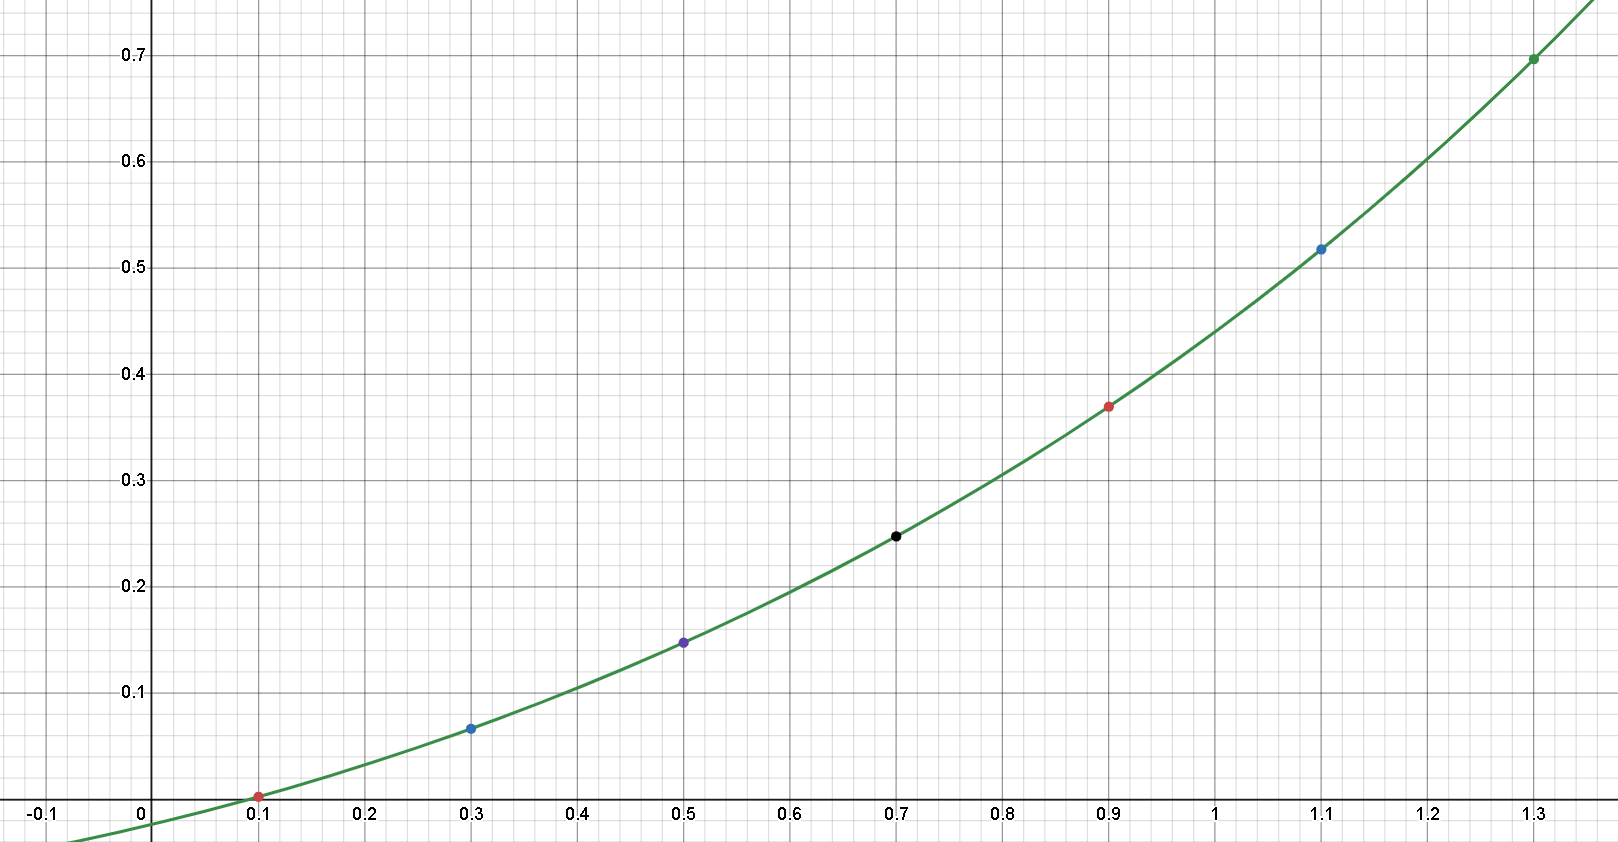
\includegraphics[width=0.75\linewidth]{image2.png}
    \caption{Plot kurva hasil estimasi menggunakan interpolasi polinom berdasarkan titik-titik yang dilewati}
\end{figure}

\pagebreak
    \item Jumlah kasus positif baru Covid-19 di Indonesia semakin fluktuatif dari hari ke hari. Di bawah ini diperlihatkan jumlah kasus baru Covid-19 di Indonesia mulai dari tanggal 17 Juni 2022 hingga 31 Agustus 2022:

    
    \begin{table}[H]
        \centering
        \caption{Tabel kasus COVID-19 17/06/2022--31/08/2022}
        \begin{tabular}{c|c|c}
             Tanggal	&	Tanggal (desimal)	&	Jumlah Kasus Baru	\\
             \hline
             \hline
$17/06/2022$	&	$6,567$	&	$12.624$	\\
$30/06/2022$	&	$7$	    &	$21.807$	\\
$08/07/2022$	&	$7,258$	&	$38.391$	\\
$14/07/2022$	&	$7,451$	&	$54.517$	\\
$17/07/2022$	&	$7,548$	&	$51.952$	\\
$26/07/2022$	&	$7,839$	&	$28.228$	\\
$05/08/2022$	&	$8,161$	&	$35.764$	\\
$15/08/2022$	&	$8,484$	&	$20.813$	\\
$22/08/2022$	&	$8,709$	&	$12.408$	\\
$31/08/2022$	&	$9$	    &	$10.534$	
        \end{tabular}
    \end{table}

    Tanggal (desimal) adalah tanggal yang sudah diolah ke dalam bentuk desimal 3 angka di belakang koma dengan memanfaatkan perhitungan sebagai berikut:

    \[ \text{Tanggal (desimal} = \text{bulan} + \text{(tanggal/jumlah hari pada bulan tersebut)} \]

    Sebagai contoh, untuk tanggal 17/06/2022 (dibaca: 17 Juni 2022) diperoleh tanggal(desimal) sebagai berikut:

    \[\text{Tanggal (desimal)} = 6 + (17/30) = 6.567 \]

    Gunakanlah data di atas dengan memanfaatkan \textbf{interpolasi polinomial} untuk melakukan prediksi jumlah kasus baru Covid-19 pada tanggal-tanggal berikut:

    \begin{enumerate}[label=(\roman*)]
        \item $16/07/2022$ (Tanggal (desimal) $= 7,5161$)
        \item $10/08/2022$ (Tanggal (desimal) $= 8,3225$)
        \item $05/09/2022$ (Tanggal (desimal) $= 9,1667$)
        \item Masukan user lainnya berupa tanggal (desimal) yang sudah diolah dengan asumsi prediksi selalu dilakukan untuk tahun 2022 (kita pilih $11/10/2022 = 10,3548$).
    \end{enumerate}

\begin{lstlisting}[caption = interpol-b.txt]
// Masukan
6.567 12.624
7.000 21.807
7.258 38.391
7.451 54.517
7.548 51.952
7.839 28.228
8.161 35.764
8.484 20.813
8.709 12.408
9.000 10.534

// Keluaran
>> Y = 7187066071652,80600 - 9346993079163,87900 X + 5334203055235,44800 X^2 - 1756810186359,80440 X^3 + 368550807175,24060 X^4 - 51131876760,09328 X^5 + 4695806315,42557 X^6 - 275474539,42049 X^7 + 9372849,23910 X^8 - 140993,71225 X^9
>> f(7,516100) = 53609,86523
>> f(8,322500) = 36433,16797
>> f(9,166700) = -664914,04688
>> f(10,354800) = -932130,96454
>> f(10,354800) = -932131180,43750\end{lstlisting}

Keluaran ini menunjukkan bahwa interpolasi polinomial dengan derajat tinggi dapat menghasilkan prediksi yang tidak realistis di luar rentang data, terutama pada tanggal yang lebih jauh dari data asli. Hal ini menunjukkan urgensi penggunaan metode lainnya, misalnya interpolasi \textit{bicubic spline}.

\pagebreak
    \item 
    
    Sederhanakan fungsi f(x) yang memenuhi kondisi
    \[ f(x) = \frac{x^2 + \sqrt{x}}{e^x + x} \]
    dengan polinom interpolasi derajat $n$ di dalam selang $[0, 2]$. Sebagai contoh, jika $n = 5$, maka titik-titik $x$ yang diambil di dalam selang $[0, 2]$ berjarak $h = (2-0)/5 = 0.4$.
\end{enumerate}

\begin{lstlisting}[caption = interpol-c.txt]
// Masukan
0 0
0.4 0.4188842
0.8 0.507157968
1.2 0.5609246748
2 0.5766515297

// Keluaran
>> Y = 0.00000 + 1,85381 X - 2,63034 X^2 + 1,68727 X^3 - 0,38174 X^4 
>> f(0,500000) = 0,45637\end{lstlisting}

Keluaran ini menunjukkan bagaimana polinom interpolasi digunakan untuk memperkirakan nilai \( f(x) \) di antara titik-titik data yang diberikan.

\begin{figure}[H]
    \centering
    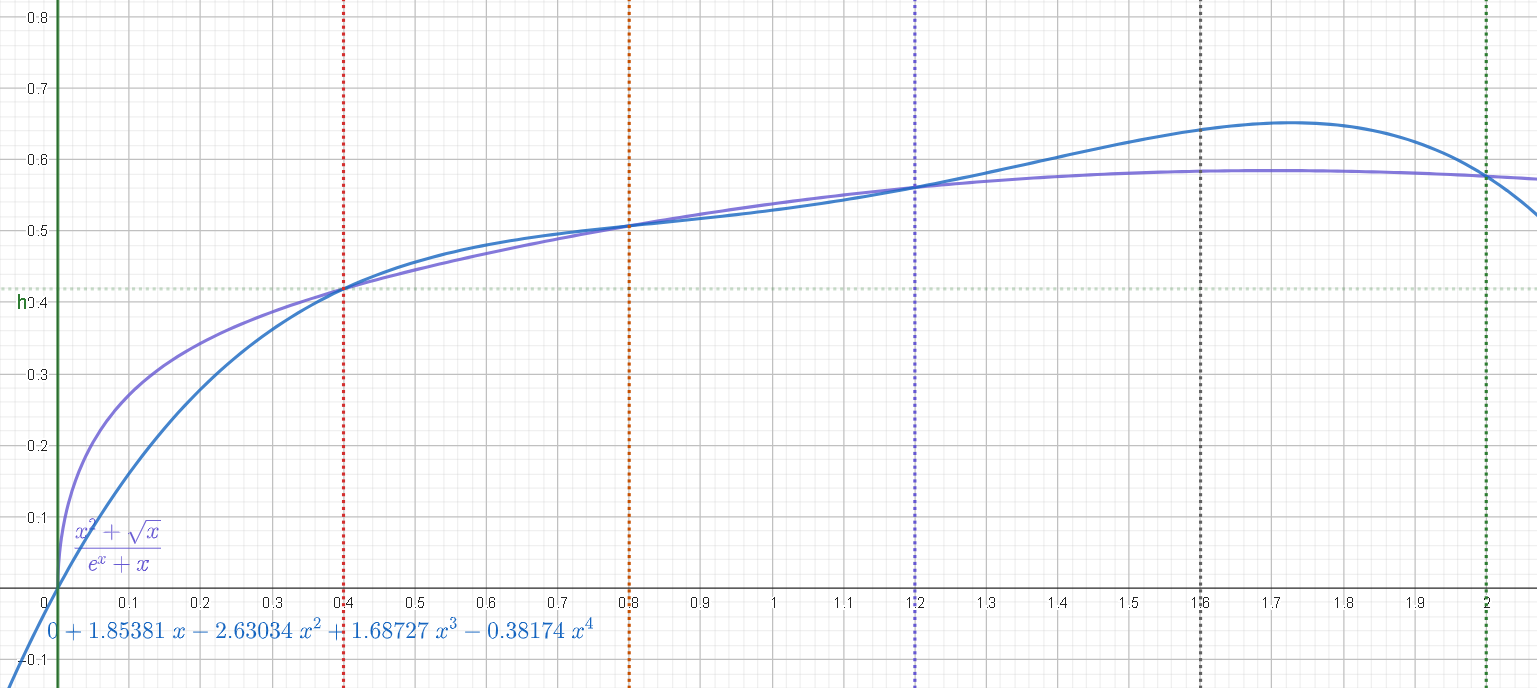
\includegraphics[width=0.75\linewidth]{image.png}
    \caption{Plot fungsi asli $f(x) = \dfrac{x^2 + \sqrt{x}}{e^x + x}$ dan fungsi hasil estimasi $g(x)$ menggunakan interpolasi polinom}
\end{figure}


\pagebreak
\subsection{Regresi Linear Berganda dan Kuadratik Berganda}
Diberikan sekumpulan data sesuai pada tabel berikut ini.\\

\begin{table}[H]
    \centering
    \caption{Data untuk studi kasus regresi linear berganda dan kuadratik berganda}
    \begin{tabular}{cccc|cccc}
        \hline
        \hline
         Nitrous Oxide, $y$ & Humidity, $x_1$ & Temp., $x_2$ & Pressure, $x_3$ &Nitrous Oxide, $y$ & Humidity, $x_1$ & Temp., $x_2$ & Pressure, $x_3$ \\
         \hline
         $0.90$ & $72.4$ & $76.3$ & $29.18$ & $1.07$ & $23.2$  & $76.8$ & $29.38$ \\
         $0.91$ & $41.6$ & $70.3$ & $29.35$ & $0.94$ & $47.4$  & $86.6$ & $29.35$ \\
         $0.96$ & $34.3$ & $77.1$ & $29.24$ & $1.10$ & $31.5$  & $76.9$ & $29.63$ \\
         $0.89$ & $35.1$ & $68.0$ & $29.27$ & $1.10$ & $10.6$  & $86.3$ & $29.56$ \\
         $1.00$ & $10.7$ & $79.0$ & $29.78$ & $1.10$ & $11.2$  & $86.0$ & $29.48$ \\
         $1.10$ & $12.9$ & $67.4$ & $29.39$ & $0.91$ & $73.3$  & $76.3$ & $29.40$ \\
         $1.15$ & $8.3$  & $66.8$ & $29.69$ & $0.87$ & $75.4$  & $77.9$ & $29.28$ \\
         $1.03$ & $20.1$ & $76.9$ & $29.48$ & $0.78$ & $96.6$  & $78.7$ & $29.29$ \\
         $0.77$ & $72.2$ & $77.7$ & $29.09$ & $0.82$ & $107.4$ & $86.8$ & $29.03$ \\
         $1.07$ & $24.0$ & $67.7$ & $29.60$ & $0.95$ & $54.9$  & $70.9$ & $29.37$ 
    \end{tabular}
\end{table}

Gunakan Normal Estimation Equation for Multiple Linear Regression untuk mendapatkan regresi linear berganda dari data pada tabel di atas, kemudian estimasi nilai \textit{Nitrous Oxide} apabila \textit{Humidity} bernilai 50$\%$, temperatur $76^\circ$F, dan tekanan udara sebesar $29.30$. 

Dari data-data tersebut, apabila diterapkan \textit{Normal Estimation Equation for Multiple Linear Regression}, maka diperoleh sistem persamaan linear sebagai berikut.

\begin{align*}
    20b_0 + 863.1b_1 + 1530.4b_2 + 587.84b_3 &= 19.42 \\
    863.1b_0 + 54876.89b_1 + 67000.09b_2 + 25283.395b_3 &= 779.477 \\
    1530.4b_0 + 67000.09b_1 + 117912.32b_2 + 44976.867b_3 &= 1483.4 \\
    587.84b_0 + 25283.395b_1 + 44976.867b_2 + 17278.5086b_3 &= 571.1219
\end{align*}

Silakan terapkan model-model ini pada Multiple Quadratic Equation juga dan bandingkan hasilnya. Sistem persamaan linear tidak akan diberikan untuk kasus ini.


\begin{lstlisting}[caption = interpol-c.txt]
// Masukan
72.40 76.30 29.18 0.90
41.60 70.30 29.35 0.91
34.30 77.10 29.24 0.96
35.10 68.00 29.27 0.89
10.70 79.00 29.78 1.00
12.90 67.40 29.39 1.10
8.30 66.80 29.69 1.15
20.10 76.90 29.48 1.03
72.20 77.70 29.09 0.77
24.00 67.70 29.60 1.07
123.20 76.80 29.38 1.07
147.40 86.60 29.35 0.94
131.50 76.90 29.63 1.10
110.60 86.30 29.56 1.10
111.20 86.00 29.48 1.10
173.30 76.30 29.40 0.91
175.40 77.90 29.28 0.87
196.60 78.70 29.29 0.78
1107.40 86.80 29.03 0.82
154.90 70.90 29.37 0.95

Query:
50 76 29.3

// Keluaran
>> Model Regresi Linear Berganda:
>> Y = 0.00000 + 1,85381 X - 2,63034 X^2 + 1,68727 X^3 - 0,38174 X^4 
>> Tes nilai (x = 0,5):
>> f(0,500000) = 0,45637

>> Model Regresi Kuadratik Berganda:
>> Y = -793,440 - 0,138X1 + 0,916X2 + 51,483X3 + 0,000X1^2 - 0,000X1X2 + 0,005X1X3 + 0,001X2^2 - 0,034X2X3 - 0,829X3^2 
>> Tes nilai (x = 0,5):
>> f(0,500000) = 0,9659864\end{lstlisting}

Keluaran menunjukkan dua model regresi yang dihasilkan dari data yang diberikan: regresi linear berganda dan regresi kuadratik berganda. Hasil dari kedua model tersebut dibandingkan dengan nilai input \( x = 0.5 \), di mana model kuadratik memberikan hasil yang sedikit lebih mendekati realitas daripada model linear.
    
\pagebreak
\subsection{Interpolasi \textit{Bicubic Spline}}

Diberikan matriks berikut,\\

\[
\begin{bmatrix}
    21 & 98 & 125 & 153 \\
    51 & 101 & 161 & 59 \\
    0 & 42 & 72 & 210 \\
    16 & 12 & 81 & 96
\end{bmatrix},
\]

tentukan nilai $f(0, 0)$, $f(0.5, 0.5)$, $f(0.25, 0.75)$, dan $f(0.1, 0.9)$.


\begin{lstlisting}[caption = interbicspl.txt]
// Masukan
21 98 125 153
51 101 161 59
0 42 72 210
16 12 81 96

// Keluaran
Masukkan titik: 0 0
>> f(0, 0) = 21
Masukkan titik: 0.25 0.74
>> f(0.25, 0.75) = 87.796875
Masukkan titik: 0.25 0.75
>> f(0.25, 0.75) = 117.732177
Masukkan titik: 0.1 0.9
>> f(0.1, 0.9) = 128.575187
\end{lstlisting}

\pagebreak
% \subsection{\textit{Image Resizing}}

\pagebreak